%% Beispiel-Präsentation mit LaTeX Beamer im KIT-Design
%% entsprechend den Gestaltungsrichtlinien vom 1. August 2020
%%
%% Siehe https://sdqweb.ipd.kit.edu/wiki/Dokumentvorlagen

%% Beispiel-Präsentation
\documentclass[en]{sdqbeamer}
 
\newcommand\blfootnote[1]{%
  \begingroup
  \renewcommand\thefootnote{}\footnote{#1}%
  \addtocounter{footnote}{-1}%
  \endgroup
}

%% Titelbild
\titleimage{unima_schloss}

%% Gruppenlogo
\grouplogo{} 

%% Gruppenname und Breite (Standard: 50 mm)
\groupname{Mannheim Master Datascience}
%\groupnamewidth{50mm}

% Beginn der Präsentation

\title[HybridBERT4Rec]{HybridBERT4Rec: A Hybrid Recommender System Based on BERT}
\subtitle{Sequential Content-Based and Collaborative Filtering}
\author[Leon Knorr]{Leon Knorr}

\date[\today]{\today}

% Literatur 
 
\usepackage[citestyle=numeric,bibstyle=numeric,hyperref,backend=biber]{biblatex}
\addbibresource{sources.bib}
\bibhang1em

\begin{document}
 
%Titelseite
\KITtitleframe

%Inhaltsverzeichnis
\begin{frame}{Table of Contents}
\tableofcontents
\end{frame}

\section{Recap}

\begin{frame}
	\centering\textbf{\LARGE{Recap: Sequential Modelling \& HybridBERT4Rec}}
\end{frame}

\subsection{Sequential Modelling}
\begin{frame}{Traditional CBF VS Sequential CBF}
	\begin{columns}
	\column{0.5\textwidth}
		\begin{figure}
			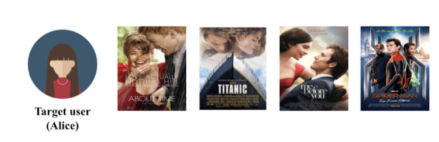
\includegraphics[width=\textwidth]{images/Alice_history.pdf}
			\caption{Example history for Alice in traditional CBF \cite{channarongHybridBERT4RecHybridContentBased2022}}
		\end{figure}
		\begin{itemize}
			\item models \textbf{general} user preference \pause
			\item \textbf{BUT:} User preferences \underline{\textbf{change over time!}} \cite{wangSequentialRecommenderSystems2019}
		\end{itemize}

	\column{.5\textwidth}
		\begin{figure}\pause
			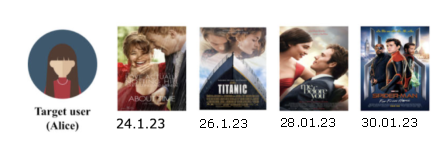
\includegraphics[width=\textwidth]{images/Alice_seq.pdf}
			\caption{Example history for Alice in sequential CBF \cite{channarongHybridBERT4RecHybridContentBased2022}}
		\end{figure}
		\begin{itemize}
			\item Considers the \textbf{order} of historical interactions
			\item Allows the modelling of \enquote{temporary spikes} of interests, as well as the general preferences \cite{wangSequentialRecommenderSystems2019}
		\end{itemize}
	\end{columns}
\end{frame}

\subsection{HybridBERT4Rec}
\begin{frame}{HybridBERT4Rec Architecture}
	\begin{figure}
		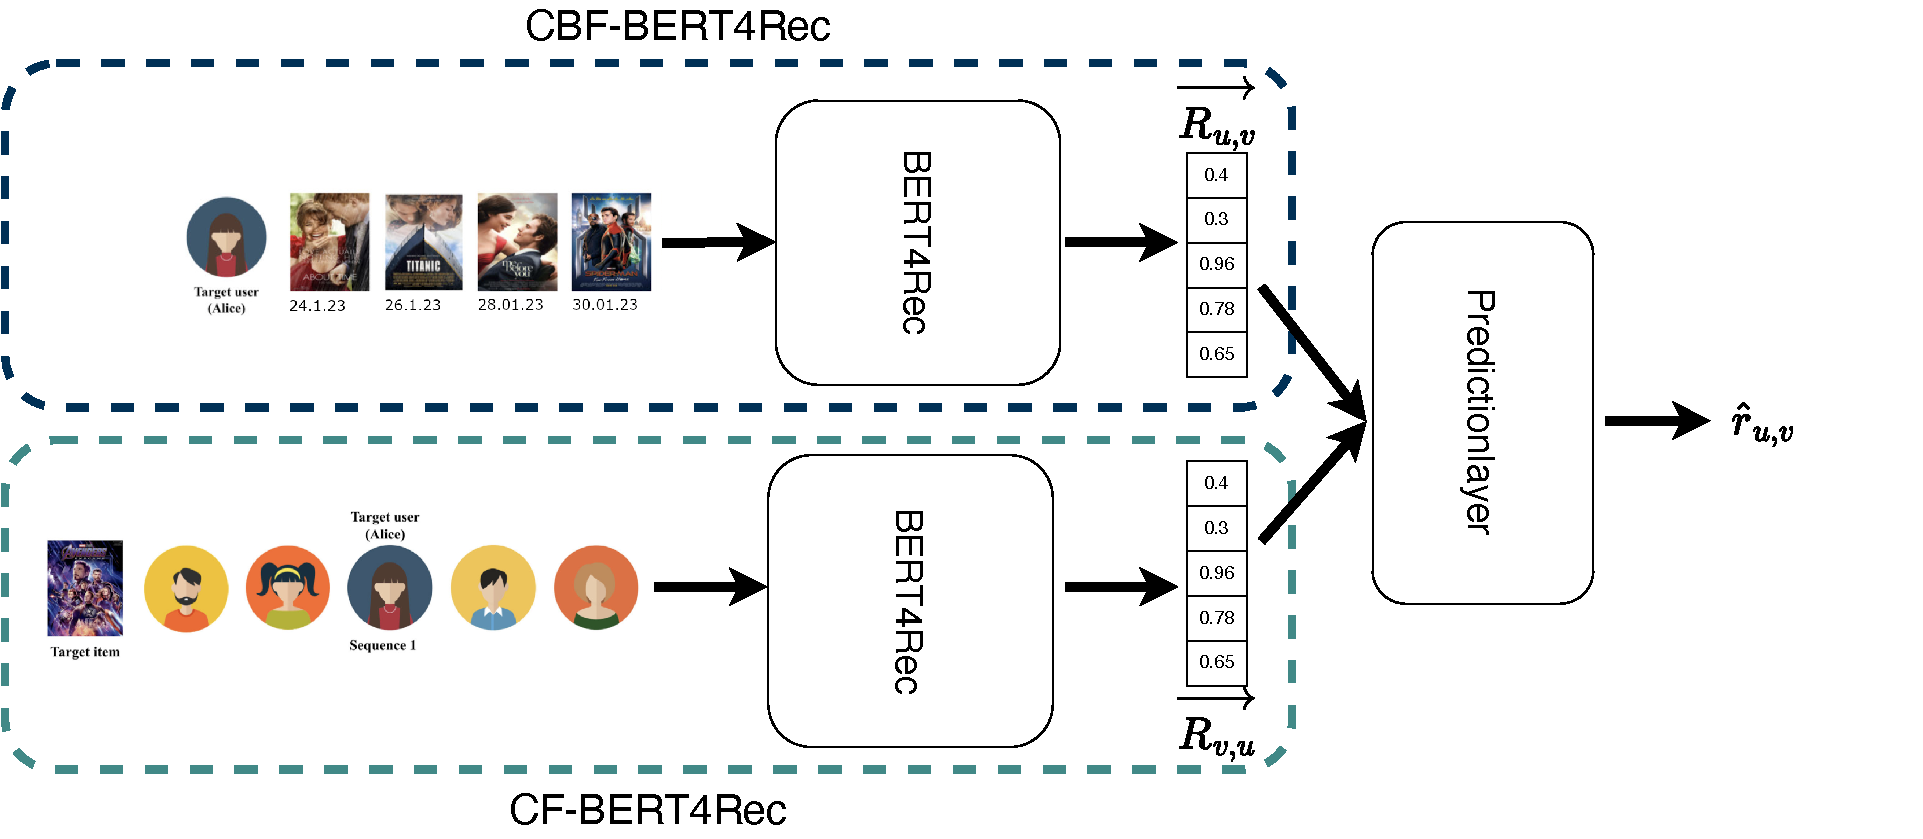
\includegraphics[height=0.6\textheight]{images/hybridBERT4Rec_high_level.pdf}
		\caption{High level overview of HybridBERT4Recs Architecture. \cite{channarongHybridBERT4RecHybridContentBased2022}}
	\end{figure}
\end{frame}

\section{The Setting}

\begin{frame}
	\centering\textbf{\LARGE{The Setting}}
\end{frame}

\begin{frame}{The Setting}
	\begin{figure}
		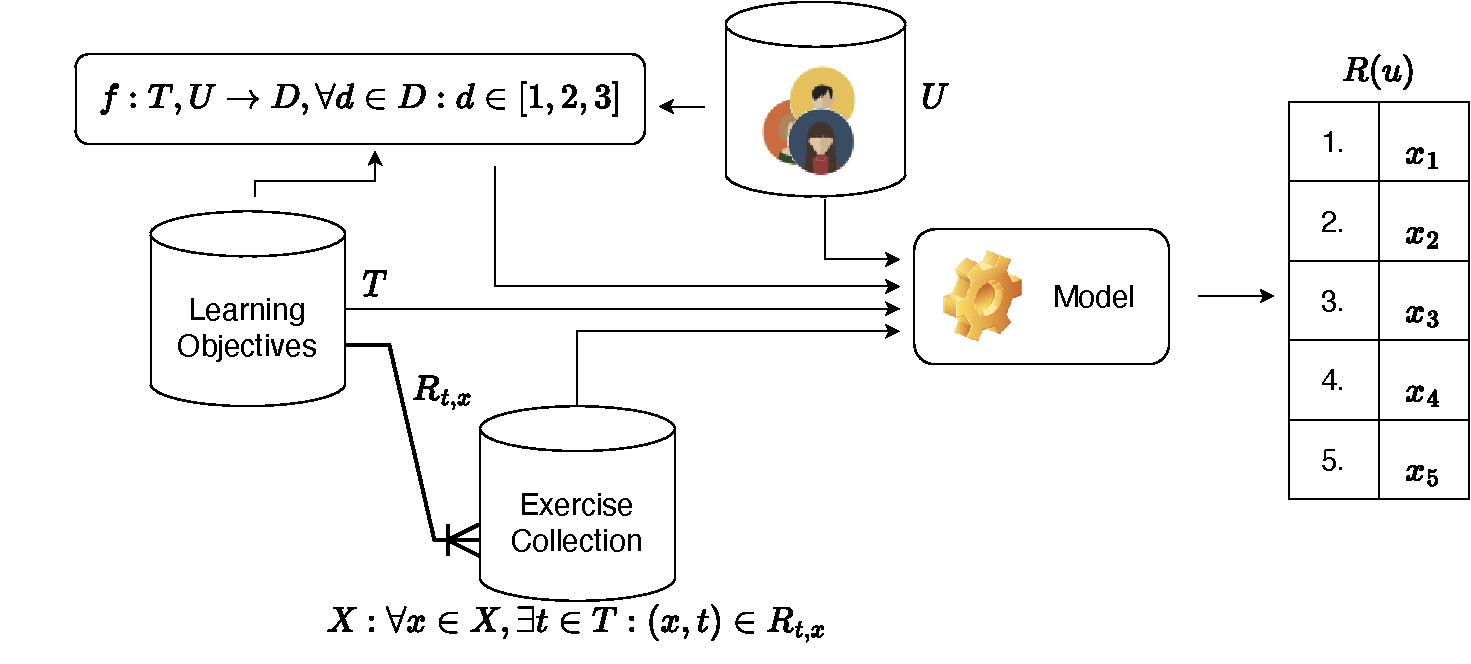
\includegraphics[height=0.6\textheight]{images/setting.pdf}
		\caption{The Setting, consisting of a user collection $U$, a collection of learning ojectives $T$ and a collection of exercises $X$, which can be used to predict a ranking $R(u)$ for a given user $u$.}
	\end{figure}
\end{frame}

\section{Model Adaption}
\begin{frame}
	\centering\textbf{\LARGE{Model Adaption}}
\end{frame}

\section{Evaluation}
\begin{frame}
	\centering\textbf{\LARGE{Evaluation}}
\end{frame}

\appendix
\beginbackup
\begin{frame}{References}
	\printbibliography
\end{frame}

\backupend

\end{document}